\section{Vypracování}
Konstrukce kartografických děl tradičně naráží na problém zkreslení, ke kterému dochází při přenosu povrchu zemského elipsoidu či sféry do roviny mapy. Jednu z cest, jak toto zkreslení minimalizovat představují polyedrické globy. Ty využívají geometrické vlastnosti platonských těles – pravidelných konvexních mnohostěnů.

Základním předpokladem pro tvorbu těchto globů je využití gnomonické projekce. V tomto zobrazení se ortodromy na sféře zobrazují jako přímky. Pokud tedy umístíme střed promítání do středu sféry vepsané danému platonskému tělesu, hranice jednotlivých stěn (plošek) tělesa vytvoří v gnomonické projekci úsečky. Díky tomu lze celou sféru rozložit na povrch mnohostěnu bez překryvů či prázdných míst.

Postup tvorby: 
\begin{itemize}
    \item Určení zeměpisných souřadnic vrcholů tělesa, které tvoří hranice pravidelných n-úhelníků (stěn).
    \item Do těžiště každé stěny je umístěn kartografický pól K, který slouží jako referenční bod pro generování sítě poledníků a rovnoběžek.
    \item Generování sítě poledníků a rovnoběžek vztažených k pólu K.
    \item Načtení bodů kontinentů a jejich následná transformace vzhledem k pólu K a obrazeny v gnomonické projekci.
    \item Oříznutí podle spojnic vrcholů n-úhelníku (platonské plošky), postup se opakuje pro všechny plošky tělesa.
\end{itemize}

Z bonusových úloh bylo zpracováno: \textbf{Výpočet meridiánové konvergence, Kontrola zkreslení v knihovně Proj} ($=5 + 15$ bodů).
\newpage
\subsection{Platonská tělesa}
Platonské těleso je pravidlený konvexní mnohostěn. 
Existuje pět platonských těles - čtyřstěn, šestistěn, osmistěn, dvanáctistěn a dvacetistěn (obrázek~\ref {ob1}).
Platí, že z každého vrcholu vychází stejný počet hran a všechny stěny tvoří shodné pravidelné mnohoúhelníky.
Každému z platonských těles lze opsat i vepsat sféru. 

 \begin{figure}[h!]
\centering
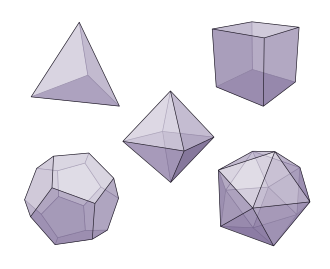
\includegraphics[scale=0.8]{figures/Platonic_Solids_Transparent.svg.png}
\captionsetup{justification=centering}
\caption{Platonská  tělesa.}
\label{ob1}
\end{figure}

\subsubsection{Šestistěn - krychle}
Krychle je tvořena šesti čtverci s délkou strany $a$. Stěnová uhlopříčka $AC$ má délku 
\[
u_s = AC = \sqrt{a^2 + a^2} =a\sqrt{2}.
\]
Tělesovou úhlopříčku lze určit z trojúhelníku $ACG$ jako 
\[
u_t = |AG| = \sqrt{u_s^2 + a^2} = \sqrt{3}a.
\]
Poloměr sféry vepsané do krychle je $r = a/2$. Úhel mezi úsečkami $AG$ a $AC$ představuje hledanou zeměpisnou šířku $u$ bodu $G$ (vrcholu)

\[
\tan u = \frac{a}{u_s} = \frac{1}{\sqrt{2}}.
\]
Vrcholy $A - D$ leží na jižní polokouli ($u_j = -u = 35,2644^\circ$), vrcholy $E-H$ leží na severní polokouli. 
Základní poledník volíme tak, aby procházel bodem $A$. Souřadnice vrcholů jsou
\[
A = [u_j, 0^\circ], \qquad
B = [u_j, 90^\circ],  \qquad
C = [u_j, 180^\circ], \qquad
D = [u_j, 270^\circ],
\]
\[
E = [u, 0^\circ], \qquad
F = [u, 90^\circ], \qquad
G = [u, 180^\circ], \qquad 
H = [u, 270^\circ]. 
\]
Kartografické póly  $K$, $L$, $M$, $N$, $S$, $J$ jsou voleny ve středech stěn krychle
\[
K = [0, 45^\circ], \qquad
L = [0, 135^\circ], \qquad
M = [0, 225^\circ], \qquad 
\]
\[
N = [0, 315^\circ], \qquad
S = [90^\circ, \cdot], \qquad
J = [-90^\circ, \cdot].
\]
\begin{figure}
    \centering
    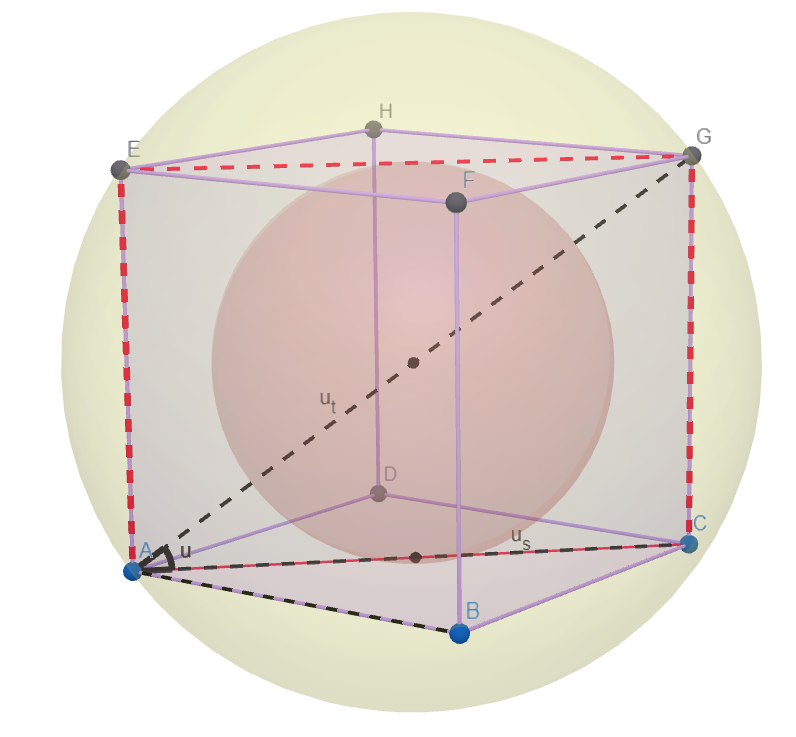
\includegraphics[width=0.7\linewidth]{figures/krzchle.png}
    \caption{Geometrie šestistěnu.}
    \label{fig:ob2}
\end{figure}


\subsubsection{Čtyřstěn}
Čtyřstěn je tvořen čtyřmi rovnostrannými trojúhelníky s délkou hrany $a$. Výšku stěny $v_s$ lze určit z trojúhelníku $A$, $E$, $D$ pomocí Pythagorovy věty
\[
v_s = |ED| = \sqrt{a^2 - \left(\frac{a}{2}\right)^2} = \frac{\sqrt{3}}{2}a.
\]
Výšky všech stěn čtyřstěnu jsou stejné, jelikož se jedná o stejné trojúhelníky. $ED$ je težnice trojúhelníku $A$, $B$, $D$, pak $|LE| = |ED|/3$. Tělesovou výšku $v_t$ lze určit z trojúhelníku $C$, $E$,
$L$ pomocí 

\[
v_t = |CL| = \sqrt{|CE|^2 - |LE|^2} = \sqrt{\frac{3}{4}a^2 -\frac{a^2}{12}} = \sqrt{\frac{2}{3}}a.
\]

Poloměr sféry vepsané do čtyřstěnu je 
\[
r = |FO|=|LE|=\frac{\sqrt{3}}{6}a.
\]
Úhel mezi úsečkami $CL$ a $CE$ představuje hledanou zeměpisnou šířku $u$ bodu $C$ (vrcholu)

\[
\sin u = \frac{|LE|}{|CE|} = \frac{|ED|}{3|ED|} =\frac{1}{3}.
\]

\begin{figure}[h!]
    \centering
    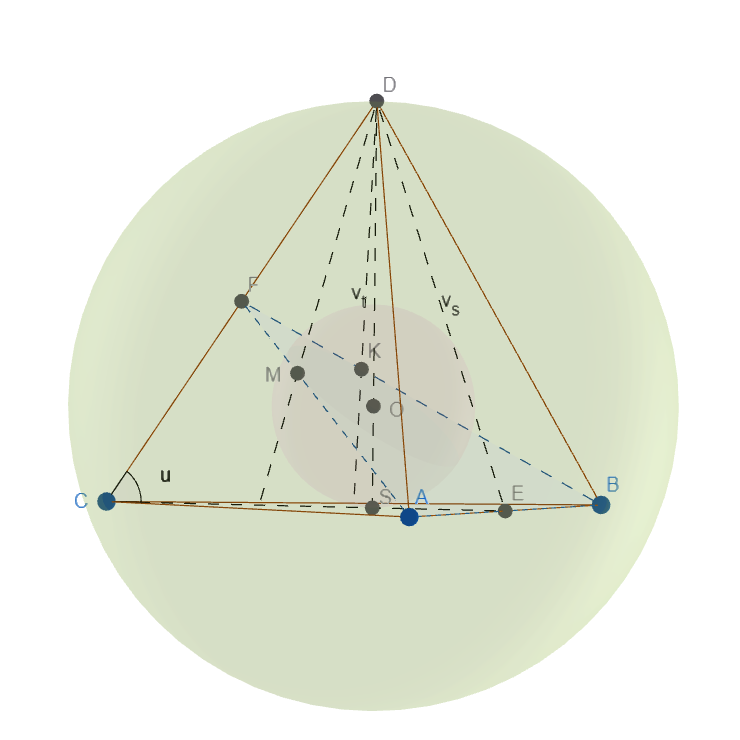
\includegraphics[width=0.5\linewidth]{figures/ctyrsten.png}
    \caption{Geometrie čtyřstěnu.}
    \label{fig:ob3}
\end{figure}


Body $A$, $B$, $C$ leží na jižní polokouli ($u_j = -u = 19,4712^\circ$).
Základní poledník volíme tak, aby procházel bodem $A$. Souřadnice vrcholů čtyřstěnu $A$, $B$, $C$, $D$ jsou
\[
A = [u_j, 0^\circ], \qquad
B = [u_j, 120^\circ],  \qquad
C = [u_j, 240^\circ], \qquad
D = [90^\circ, \cdot].
\]
Kartografický pól leží v těžišti každé plošky čtyřstěnu, jeho zeměpisná šířka $u_k$ je pro šikmé plošky rovna $u_k= u$, pro podstavu $u_k = -90^\circ$.
Zeměpisné souřadnice kartografických pólů $K$, $L$, $M$, $N$ jsou
\[
K = [u, 60^\circ], \qquad
L = [u, 180^\circ], \qquad
M = [u, 300^\circ], \qquad 
N = [-90^\circ, \cdot]. 
\]

\subsubsection{Osmistěn}
Osmistěn je tvořen osmmi rovnostrannými trojúhelníky s délkou hrany $a$. Výšku stěny $v_s$ lze určit z trojúhelníku $E$, $G$, $C$ pomocí Pythagorovy věty
\[
v_s = |EG| = \sqrt{a^2 - \left(\frac{a}{2}\right)^2} = \frac{\sqrt{3}}{2}a.
\]
Tělesová úhlopříčka je úhlopříčka čtverce se stranou $a$

\[
v_t = |AC| = \sqrt{2}\cdot a.
\]

Poloměr sféry vepsané do osmistěnu je 
\[
r = \sqrt{|OG|^2 - |IG|^2}=\sqrt{\frac{a^2}{4}-\frac{1}{12}a^2}=\frac{a}{\sqrt{6}}.
\]

Úhel mezi úsečkami $OI$ a $OG$ představuje hledanou zeměpisnou šířku $u$ bodu $I$ (vrcholu)

\[
\sin u = \frac{|IG|}{|OG|} = \frac{\sqrt{3}a/{6}}{{a}/{2}} =\frac{\sqrt{3}}{3},
\]
kde $u = 35,2644^\circ$.

\begin{figure}[h!]
    \centering
    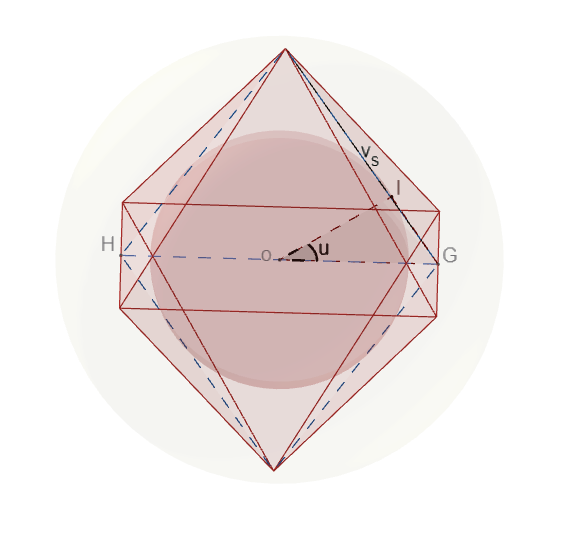
\includegraphics[width=0.7\linewidth]{figures/osmisten.png}
    \caption{Geometrie osmistěnu.}
    \label{fig:ob4}
\end{figure}


Body $A-D$ leží na rovníku, body $E$ a $F$ jsou póly
\[
A = [0^\circ, 0^\circ], \quad
B = [0^\circ, 90^\circ],  \quad
C = [0^\circ, 180^\circ], \quad
D = [0^\circ, 270^\circ], \quad
E = [90^\circ, \cdot], \quad
F = [-90^\circ, \cdot].
\]
Kartografické póly $I-P$ leží v těžištích každé plošky osmistěnu.
Póly $I$, $J$, $K$, $L$ leží na severní polokouli
\[
I = [u, 45^\circ], \qquad
J = [u, 135^\circ], \qquad
K = [u, 225^\circ], \qquad 
L = [u, 315^\circ]. 
\]
Póly $M$, $N$, $O$, $P$ leží na jižní polokouli
\[
M = [-u, 45^\circ], \qquad
N = [-u, 135^\circ], \qquad
O = [-u, 225^\circ], \qquad 
P = [-u, 315^\circ]. 
\]

\newpage
\subsection{Gnomonická projekce}
Gnomonická projekce patří mezi azimutální zobrazení. Středem promítání (okem pozorovatele) je samotný střed sféry $C$. Body z povrchu koule promítáme na rovinu, která je tečná ke sféře v kartografickém pólu $K$. V nejčastěji uváděné normální poloze splývá kartografický pól se severním zeměpisným pólem ($K\equiv
S$).
\begin{figure}[h!]
    \centering
    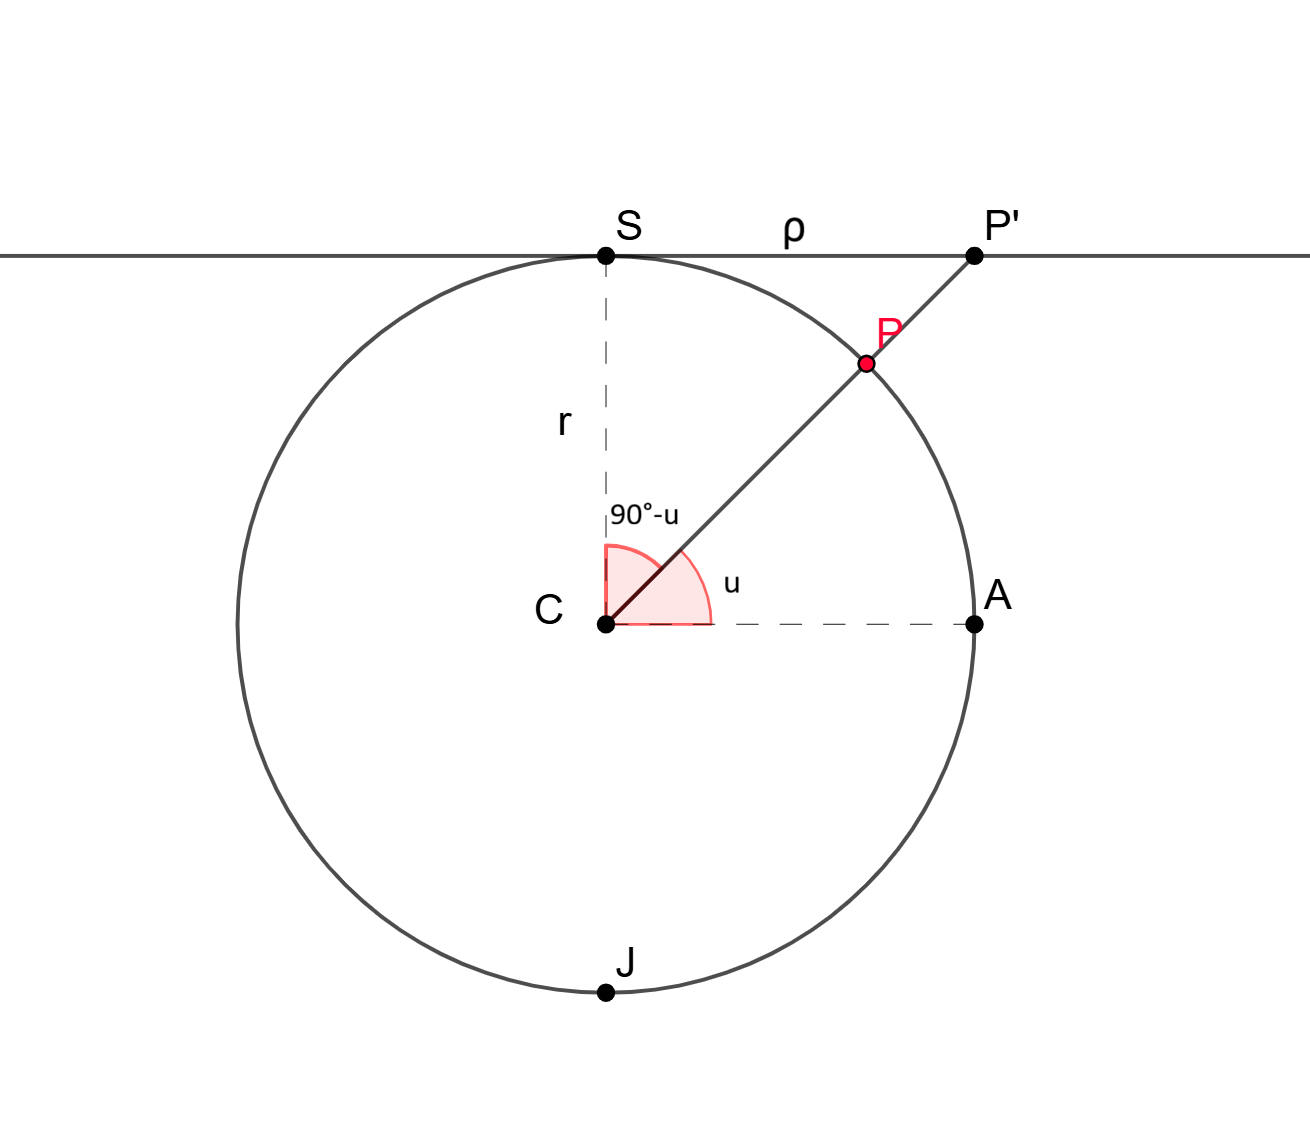
\includegraphics[width=0.7\linewidth]{figures/gnom.png}
    \caption{Gnomonická projekce v normální poloze.}
    \label{fig:ob5}
\end{figure}

Z geometrie zobrazení (viz pravoúhlý trojúhelník $SCP'$  na obrázku~\ref{fig:ob5}) vyplývá, že obraz $P'$ bodu $P$ leží na rovnoběžkové kružnici $k(S,\rho)$ o poloměru $\rho=|SP'|$. Zobrazovací rovnice v polárním tvaru lze zapsat jako:
\begin{align*}
\rho &= r \cdot \tan (90^{\circ} - \textit{u}), \\
\epsilon &= v,
\end{align*}
kde $r$ představuje poloměr sféry, $u$ je zeměpisná šířka bodu, $v$ je zeměpisná délka bodu.

V obecné poloze, vztažené ke kartografickému pólu $K=[u_k,v_k]$, nabývají rovnice v polárních souřadnicích tvaru:
\begin{align*}
\rho &= r \cdot \tan (90^{\circ} - \textit{š}), \\
\epsilon &= d,
\end{align*}

kde $š$ a $d$ jsou kartografická šířka a délka bodu. 
Pro převod do pravoúhlé souřadnicové soustavy ($x$,$y$) pak platí:
\begin{align*}
x &= R \cdot \tan (90^{\circ} - \textit{š}) \cdot \cos d, \\
y &= R \cdot \tan (90^{\circ} - \textit{š}) \cdot \sin d.
\end{align*}
Gnomonická projekce vyniká unikátní vlastností: obrazem každé ortodromy (hlavní kružnice na kouli) je přímka. Jelikož poledníky tvoří ortodromy, jejich obrazy jsou polopřímky vycházející z pólu. Obrazy rovnoběžek jsou pak kružnice (v normální poloze) nebo jiné kuželosečky (v obecné poloze).

Z limitního chování funkce tangens vyplývá zásadní omezení:
\[
\lim_{u \to \pm 0} \tan(90^\circ - u) = \pm \infty.
\]
Z toho je patrné, že gnomonická projekce není schopna zobrazit celou polokouli. V praxi lze zobrazit pouze část sféry; rovník se v normální poloze promítá do nekonečna, a proto musí být z mapy vždy vyjmut.
\newpage
\subsubsection{Vlastnosti projekce}
V této částo definujeme vlastnosti gnomonické projekce, a to: 
\begin{itemize}
    \item měřítko $m_p$ v poledníku, měřítko $m_r$ v rovnoběžce,
    \item poloosy $a$, $b$ Tissotovy indikatrix,
    \item úhel $\omega'$ mezi obrazem poledníku a rovnoběžky,
    \item maximální úhlové zkreslení $\Delta\omega$,
    \item měřítko ploch $P$,
    \item meridiánová konvergence $c$.
\end{itemize}
První krok, který je nutný provést je určení parciální derivace zobrazovacích rovnic podle jednotlivých proměnných.
\begin{align*}
\frac{\partial f}{\partial u} &= f_u = - \frac{R}{\cos^2 (90^\circ - u)} \cos v, \\
\frac{\partial f}{\partial v} &= f_v = -R \tan(90^\circ - u)\sin v,\\
\frac{\partial g}{\partial u} &= g_u = - \frac{R}{\cos^2 (90^\circ - u)} \sin v,\\
\frac{\partial g}{\partial v} &= g_v = R \tan(90^\circ - u)\cos v.
\end{align*}
Měřítko v poledníku $m_p$ je pak dáno vztahem
\[
m_p^2 = \frac{f_u^2+g_u^2}{R^2},
\]
po dosazení parciálních derivací a upravení získáme
\[
m_p = \frac{1}{\sin^2u}.
\]
Měřítko v rovnoběžce $m_r$ je dáno vztahem 
\[
m_r^2 = \frac{f_v^2+g_v^2}{R^2\cos^2u},
\]
po dosazení parciálních derivací a upravení získáme
\[
m_r = \frac{1}{\sin u}.
\]
Pro poloosy $a$, $b$ Tissotovy indikatrix platí
\[
a= m_p, \qquad \qquad b= m_r.
\]
Úhel $\omega'$ mezi obazem poledníku a rovnoběžky je dán vztahem
\[
\tan\omega' = \frac{g_uf_v-f_ug_v}{f_uf_v+g_ug_v}
\]
po úpravě získáme
\[
\omega' = \pm \frac{\pi}{2}= 90^\circ.
\]
Maximální úhlové zkreslení $\Delta\omega$ je vyjádřeno
\[
\sin\frac{\Delta\omega}{2}=\frac{|b-a|}{b+a}=\frac{|m_r-m_p|}{m_r+m_p},
\]
po dosazení a upravení získáme
\[
\sin\frac{\Delta\omega}{2}=\frac{1-\sin u}{1+\sin u}.
\]
Měřítko ploch $P$ je dáno vztahem
\[
P = \frac{g_uf_v-f_ug_v}{R^2\cos u},
\]
po dosazení a upravení získáme
\[
P=\frac{1}{\sin ^3u}.
\]
Meridiánová konvergence $c$ je definována vztahem 
\[
\tan\sigma_p = \frac{g_u}{f_u},
\]
dosazením a upravením získáme 
\[
\sigma_p = v.
\]

\subsection{Konstrukce globů}
Všechny potřebné skripty pro konstrukci globů byly vytvořeny v prostředí SW MATLAB. Celý proces je logicky rozdělen do dílčích funkcí, které na sebe navazují – od základních transformací souřadnic přes generování prvků mapy až po finální vizualizaci a výpočet zkreslení.

\textbf{Transformace souřadnic:} Základem je skript \lstinline{uvTosd.m}, který zajišťuje převod zeměpisných souřadnic na souřadnice kartografické. Na něj navazuje funkce \lstinline{gnom.m}, jež obsahuje samotné zobrazovací rovnice gnomonické projekce a transformuje zeměpisné souřadnice do pravoúhlé soustavy.

\textbf{Generování obsahu plošek:} Skript \lstinline{graticule.m} vypočítává souřadnice geografické sítě pro konkrétní plošku tělesa. Zásadní je zde  ošetření zobrazení sítě, aby nedocházelo k chybám při projekci do nekonečna. Pro zákres pevniny slouží funkce \lstinline{drawContinent.m}. Ta načítá souřadnice z textových souborů, transformuje je a zároveň filtruje body ležící příliš blízko rovníku, jelikož ty v gnomonické projekci nelze zobrazit.

\textbf{Kompletace a ořez:} Pro správný vzhled polyedrického globu vytváří skript \lstinline{boundary.m} ořezové hranice odpovídající tvaru dané platonské plošky. Hlavní vykreslovací funkce \lstinline{createGlobeFace.m} následně všechny tyto vrstvy (síť, kontinenty a hranice) spojí a vizualizuje.

\textbf{Analýza zkreslení:} Skript \lstinline{gnom_distortions.m} provádí analytické výpočty vlastností projekce, včetně měřítek a plošného zkreslení. Vizuální reprezentaci těchto deformací řeší funkce \lstinline{elipse_Tissot.m}. Protože MATLAB nedisponuje nativní funkcí pro přímé vykreslení elipsy v daných parametrech, algoritmus nejprve generuje elipsu v počátku souřadnicového systému a až poté ji pomocí maticové rotace a translace umisťuje do požadované pozice.

Pro každé z testovaných těles (čtyřstěn, šestistěn, osmistěn) existuje samostatná sada zastřešujících skriptů uložená v příslušné složce, která zajišťuje postupné vygenerování všech potřebných stěn.



\newpage
\section{Výsledky}
\subsection{Vlastnosti gnomonické projekce}
V tabulce~\ref{table:1} jsou uvedeny hodnoty vypočítaných parametrů z SW MATLAB. 
K porovnání jsou ty samé parametry spočítany pomocí knihovny Proj (tabulka~\ref{table:2} ).

\begin{table}[htbp]
\centering
\renewcommand{\arraystretch}{1.2} 
\begin{tabular}{|r||c|c|c|}
\hline
 & čtyřstěn & šestistěn & osmistěn \\
\hline
měřítko $m_p$ v poledníku & 9.000018 & 2.999998 & 1.500000 \\
\hline
měřítko $m_r$ v rovnoběžce & 3.000003 & 1.732050 & 1.224745 \\
\hline
poloosa $a$ & 9.000018 & 2.999998 & 1.500000 \\
\hline
poloosa $b$ & 3.000003 & 1.732050 & 1.224745 \\
\hline
úhel $\omega'$ mezi obrazem poledníku a rovnoběžky & $\mp$ 90$^\circ$ & $\mp$ 90$^\circ$ & $\mp$ 90$^\circ$ \\
\hline
maximální úhlové zkreslení $\Delta\omega$ & 60$^\circ$ 0' 0'' & 31$^\circ$ 5' 4'' & 11$^\circ$ 35' 4'' \\
\hline
měřítko ploch $P$ & 27.000083 & 5.196148 & 1.837118 \\
\hline
meridiánová konvergence $c$ & 90$^\circ$ & 90$^\circ$ & 90$^\circ$ \\
\hline

\end{tabular}
\caption{Výsledné hodnoty parametrů gnomonické projekce (MATLAB).}
\label{table:1}
\end{table}


\begin{table}[htbp]
\centering
\renewcommand{\arraystretch}{1.2} 
\begin{tabular}{|r||c|c|c|}
\hline
 & čtyřstěn & šestistěn & osmistěn \\
\hline
měřítko $m_p$ v poledníku & 9.000018 & 2.999998 & 1.500000 \\
\hline
měřítko $m_r$ v rovnoběžce & 3.000003 & 1.732050 & 1.224745 \\
\hline
poloosa $a$ & 9.000018 & 2.999998 & 1.500000 \\
\hline
poloosa $b$ & 3.000003 & 1.732050 & 1.224745 \\
\hline
úhel $\omega'$ mezi obrazem poledníku a rovnoběžky & $\mp$ 90$^\circ$ & $\mp$ 90$^\circ$ & $\mp$ 90$^\circ$ \\
\hline
maximální úhlové zkreslení $\Delta\omega$ & 60$^\circ$ 0' 0'' & 31$^\circ$ 5' 4'' & 11$^\circ$ 35' 4'' \\
\hline
měřítko ploch $P$ & 27.000083 & 5.196148 & 1.837118 \\
\hline
meridiánová konvergence $c$ & 90$^\circ$ & 90$^\circ$ & 90$^\circ$ \\
\hline
\end{tabular}
\caption{Výsledné hodnoty parametrů gnomonické projekce (Proj).}
\label{table:2}
\end{table}

V tabulce~\ref{table:1} jsou uvedeny hodnoty parametrů vypočítaných pomocí navržených algoritmů v SW MATLAB. Pro verifikaci správnosti matematického modelu byly tytéž parametry podrobeny kontrole pomocí zavedené kartografické knihovny Proj (tabulka~\ref{table:2}). Hodnoty získané z obou softwarových řešení jsou zcela totožné, z čehož lze usoudit, že implementace výpočtů v prostředí MATLAB je korektní.

Z vypočtených dat (viz tabulky)  je zřejmý přímý vliv typu použitého mnohostěnu na míru zkreslení v okrajovém bodě stěny. Lze pozorovat, že s rostoucím počtem stěn tělesa (a tím pádem menší plochou jedné stěny) se radikálně snižuje jak maximální úhlové zkreslení ($\Delta\omega)$, tak plošné měřítko ($P$). Zatímco u čtyřstěnu dosahuje úhlové zkreslení v okrajovém bodě extrémní hodnoty $60^\circ0'$0" a plocha je zvětšena zhruba 27krát, u osmistěnu úhlové zkreslení klesá na přijatelnějších $11^\circ35'$4" s plošným zkreslením necelého dvojnásobku.

\newpage
\subsection{Tissotovy elipsy}

\begin{figure}[htbp]
    \centering
    
    \begin{subfigure}{0.45\textwidth}
        \centering
        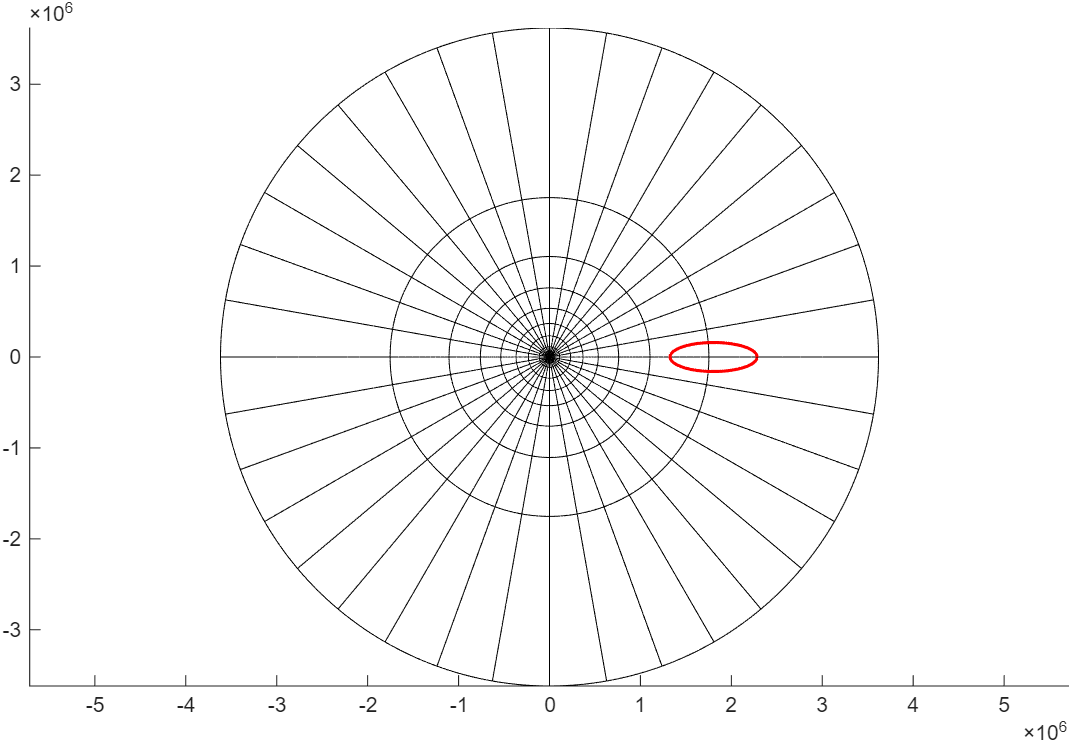
\includegraphics[width=\textwidth]{figures/tiss_tetra.png} 
        \caption{}
        \label{fig:top_left}
    \end{subfigure}
    \hfill 
    \begin{subfigure}{0.45\textwidth}
        \centering
        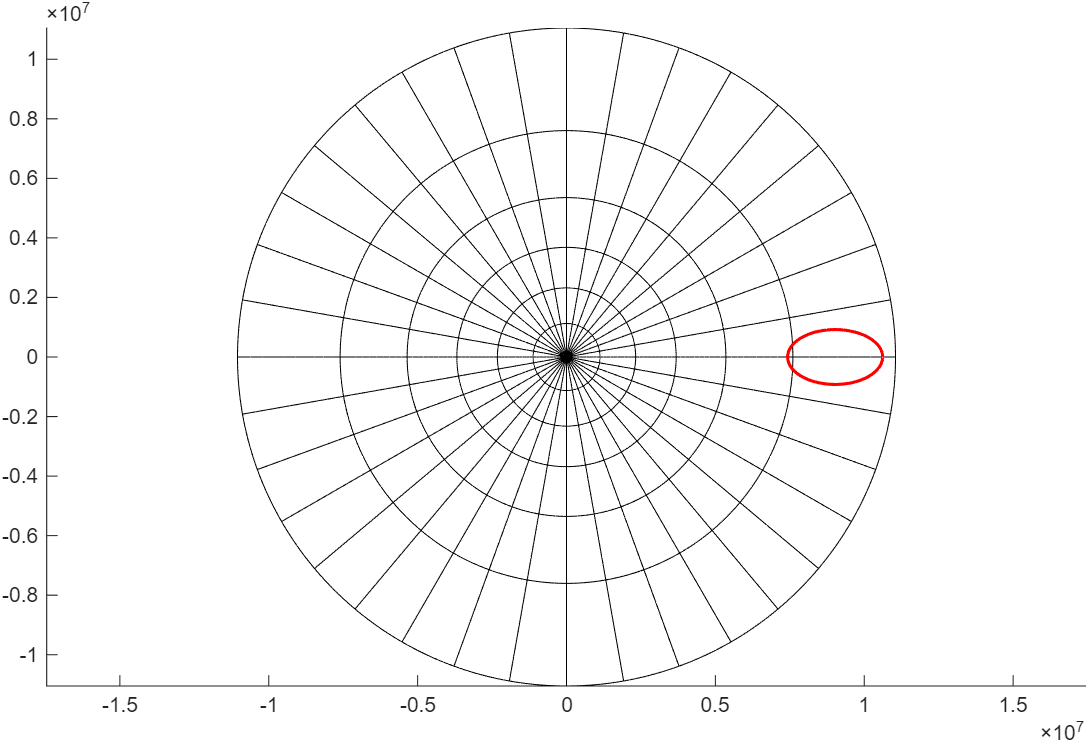
\includegraphics[width=\textwidth]{figures/tiss_cube.png} 
        \caption{}
        \label{fig:top_right}
    \end{subfigure}
    
    \vspace{1em} 
    
    
    \begin{subfigure}{0.45\textwidth}
        \centering
        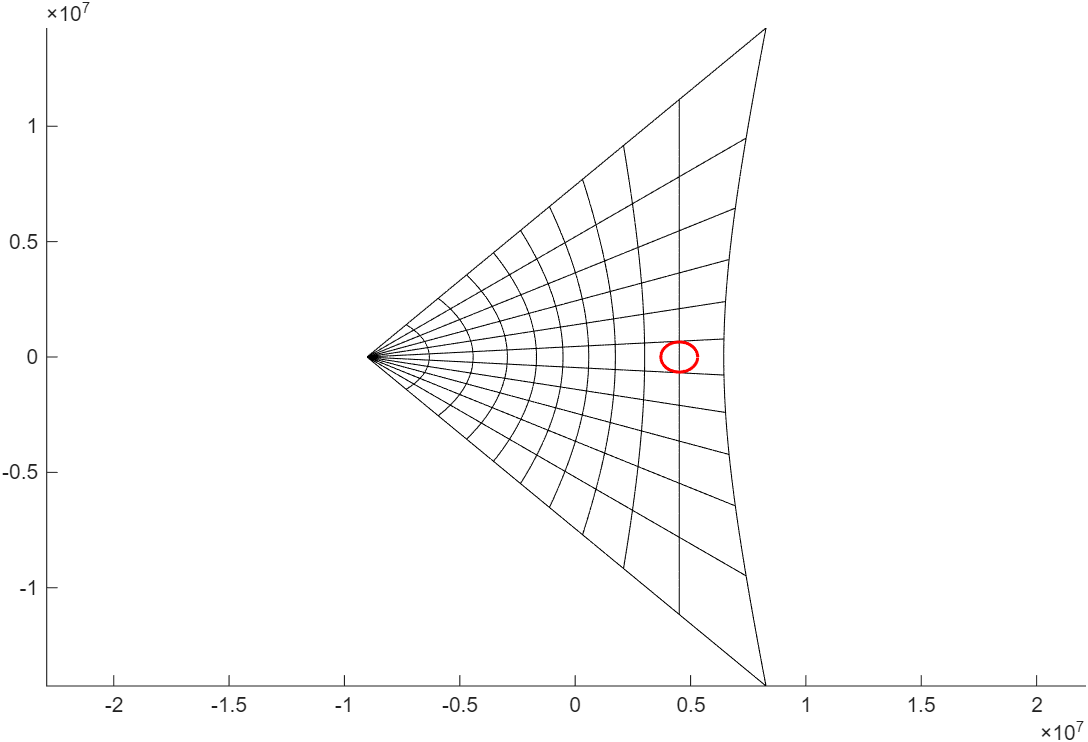
\includegraphics[width=\textwidth]{figures/tiss_octa.png} 
        \caption{}
        \label{fig:bottom_center}
    \end{subfigure}
    
    \caption{Tissotovy elipsy - čtyřstěn (a), šestistěn (b), osmistěn (c).}
    \label{fig:three_images}
\end{figure}

Obrázek~\ref{fig:three_images} ilustruje tvar a velikost Tissotových elips pro jednotlivá zkoumaná tělesa: čtyřstěn (a), šestistěn (b) a osmistěn (c). Tissotova indikatrix poskytuje názornou vizuální reprezentaci úhlového a plošného zkreslení, které bylo kvantifikováno v předchozí kapitole.

Ve středu každé plošky (v místě dotyku referenční sféry a roviny projekce) nedochází ke zkreslení a indikatrix by měla tvar dokonalé kružnice. Vlivem gnomonické projekce se však směrem k okrajům (vrcholům platonských těles) plošky rapidně protahují a zvětšují. Z grafických výstupů je jasně patrné, že elipsa vykreslená pro čtyřstěn (a) vykazuje největší protažení i nárůst plochy, což plně koresponduje s vypočtenými hodnotami $m_p$, $m_r$ a $P$ z tabulek. Naopak elipsa u osmistěnu (c) si zachovává tvar nejpodobnější kružnici, což vizuálně potvrzuje, že aproximace sféry pomocí tělesa s více stěnami je z hlediska minimalizace okrajových deformací efektivnější.


\section{Závěr}
Hlavním cílem této úlohy byla polyedrická aproximace sféry pomocí vybraných platonských těles. Celý proces zpracování, zahrnující matematickou definici těles, generování geografické sítě, projekci kontinentů v gnomonickém zobrazení a výpočet deformací, byl úspěšně proveden ve skriptovacím jazyce programu MATLAB.

Z provedených výpočtů i vizualizací Tissotových elips jednoznačně vyplývá, že míra zkreslení gnomonické projekce roste se vzdáleností od kartografického pólu (středu plošky). Z porovnávaných platonských těles se jako nejvhodnější varianta jeví osmistěn, který díky většímu počtu stěn a jejich menší ploše efektivně minimalizuje extrémní úhlové i plošné deformace, ke kterým dochází zejména u čtyřstěnu.